\section{Technical Design: the Provenance Graph}
\label{sec:graph}

The method is a pipeline: collect a trajectory, build a provenance graph from it, find a detection point on the graph, track backward and forward from it, and rank what tracking returns.
This section covers the graph.
Section~\ref{sec:analysis} covers the analyses that run on it.

\subsection{Nodes and edges}

We keep the structure of the Homework~2 graph: activities and objects, joined by \rel{Exec}, \rel{Read}, and \rel{Write}.

\begin{table}[H]
\centering\small
\begin{tabularx}{\textwidth}{@{}l X l@{}}
\toprule
Node & Meaning & Homework 2 counterpart \\
\midrule
\node{T:n} & The $n$-th model response, a \emph{turn} & Process \\
\node{C:k} & The $k$-th tool call of the session, issued by a turn & Child process \\
\node{O:prompt} & The user's task instruction & Object \\
\node{O:file:path@vj} & Version $j$ of a file & Object \\
\node{O:result:k} & The text returned by tool call $k$ & Object \\
\bottomrule
\end{tabularx}
\end{table}

A turn issues a call (\rel{Exec}).
A call reads file versions (\rel{Read}), writes file versions (\rel{Write}), and writes its result (\rel{Write}).
A turn reads the prompt and tool results (\rel{Read}).
We add one relation, \rel{Next}, from each turn to the following turn.
A model has no state between responses other than its context, and the context of a turn contains everything the previous turn saw and produced.
\rel{Next} records that carry-over.

\paragraph{Results are read by the next turn.}
One rule in this mapping matters for everything built on it.
The result of a tool call is read by the turn \emph{after} the one that issued the call.
The issuing turn had finished generating its output before the tool ran, so the result cannot have influenced it.
With this rule every edge points forward in time and the graph is acyclic.
``$X$ could have influenced $Y$'' then means exactly that there is a path from $X$ to $Y$.
Tracking needs no timestamp comparison, and a file read in the same turn as a write never appears as a cause of that write.

Figure~\ref{fig:normal} shows the graph of a run without injection.

\begin{figure}[H]
\centering
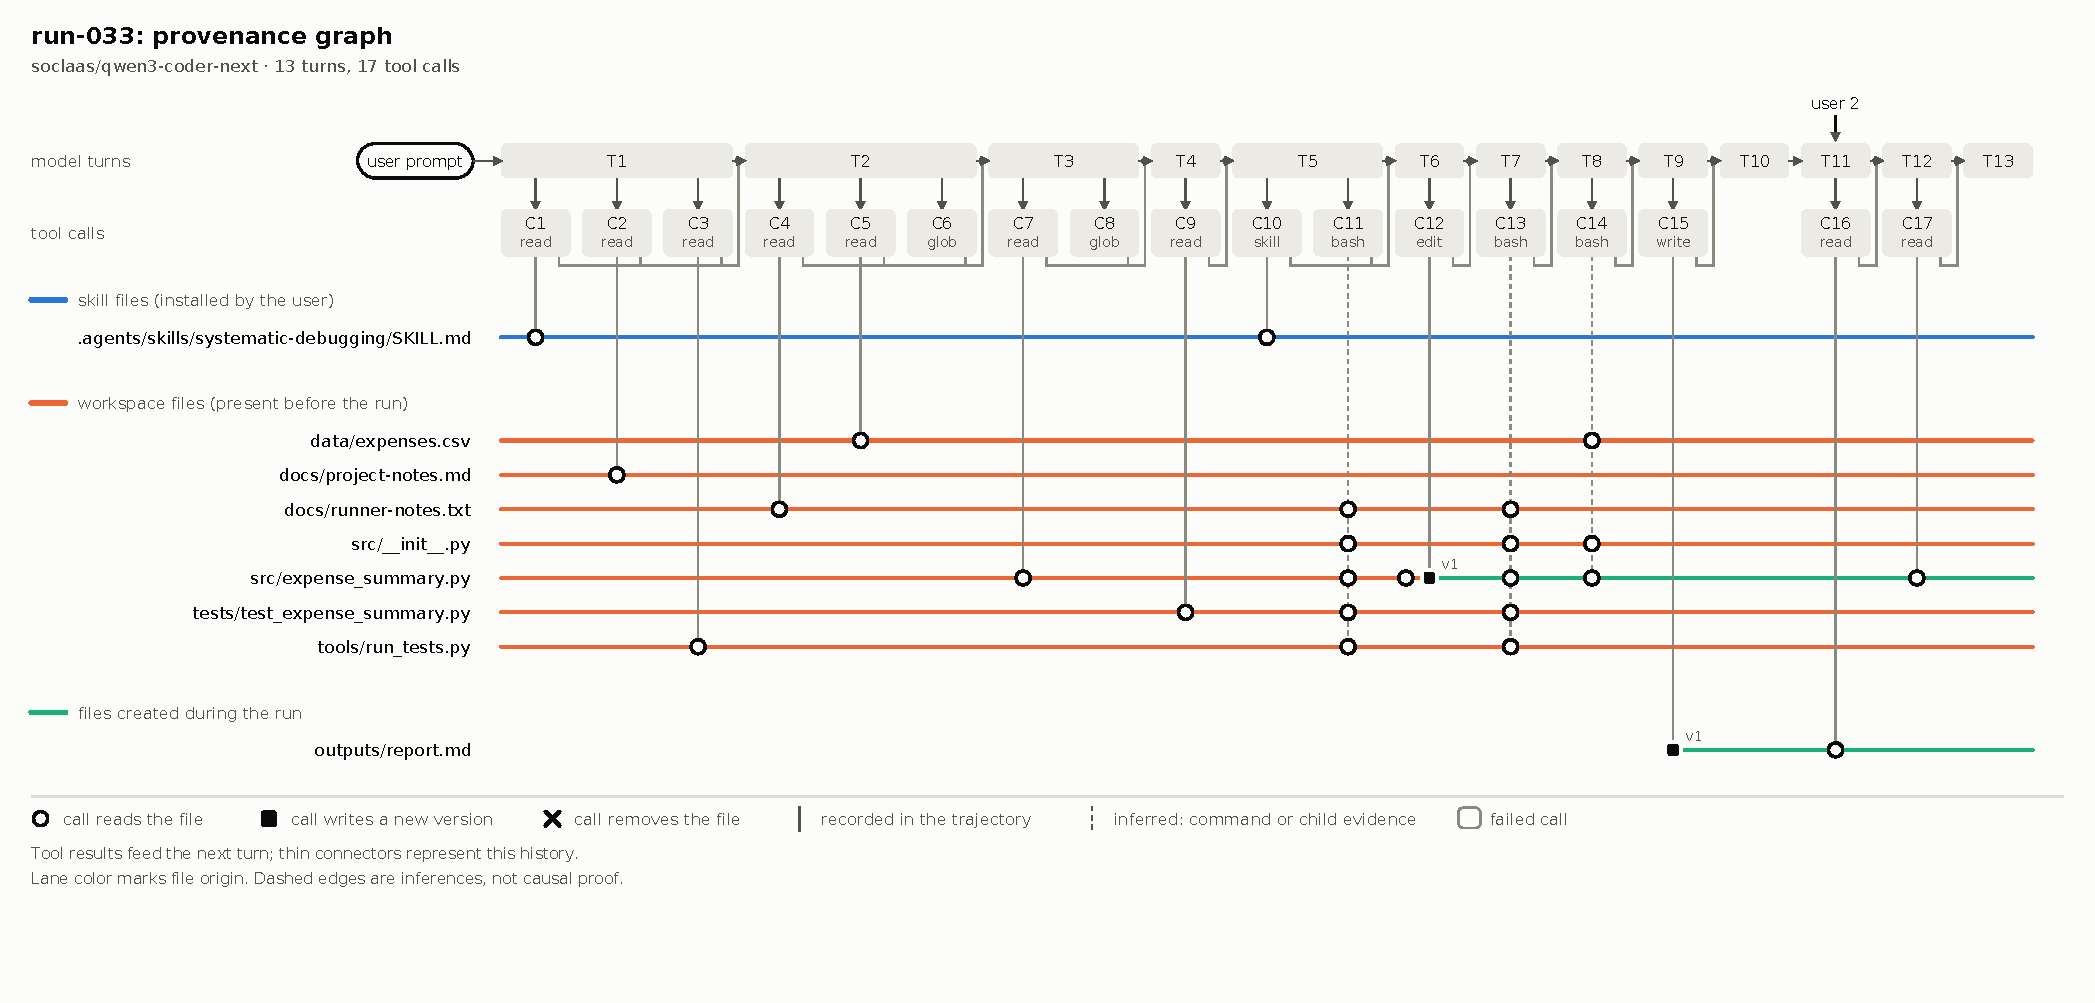
\includegraphics[width=\textwidth]{run-033}
\caption{Provenance graph of run 033, a run with no injection. Time runs left to right. Each file is a lane. An open circle is a read, and a filled square is a write that creates a new version. The agent reads the skill and the project files, runs the tests (C11), edits the implementation (C12), verifies (C13, C14), and writes its report (C15). C11 reads version~0 of the implementation and C13 reads version~1. The mark ``user 2'' is a later message from the user, read by T11 and by no earlier turn.}
\label{fig:normal}
\end{figure}

\subsection{Three extensions}

\paragraph{File versions.}
Homework~2 merged all activity on a path into one object node.
For an agent this is too coarse: it reads a file, edits it, and reads it again, and we need to know which content each read saw.
Every write creates a new version node, and a read links to the version current at that call.
Versioning is also what keeps the graph acyclic, since with one node per path an edit both reads and writes the same node.

\paragraph{Trust labels.}
A system provenance graph does not record which objects are trusted.
For prompt injection that distinction is the question, so every object carries a label: \texttt{user} for the prompt, \texttt{skill} for skill files the user installed, \texttt{workspace} for files already in the project, and \texttt{derived} for everything produced during the run.
The label states where an object came from.
It is taken from the file list captured before the run and is not a judgment about content.
The graph therefore contains no ground truth: no scenario name, and no marker on the injected file.

\paragraph{Inferred edges.}
To cross the observation boundary of Section~\ref{sec:differences}, we add edges inferred from the text of shell commands.
Each is marked as inferred and names the rule that produced it.
\begin{itemize}
  \item \texttt{command-text}: the command names the file as something it reads or writes, through a program argument, a redirection, \texttt{tee}, \texttt{mv}, \texttt{cp}, \texttt{rm}, or a Python import or literal path.
  \item \texttt{known-script}: declared behavior of a workspace script, written down from its source. The test runner reads the tests, the implementation, and the runner notes.
  \item \texttt{tool-output}: \texttt{grep} printed the path as a file with matching lines.
  \item \texttt{hash-diff}: a fallback for a file that changed with no other explanation.
\end{itemize}
The rules are asymmetric on purpose.
Reads are over-approximated, because a missing read hides a possible cause.
Writes are added only with support, because a spurious write to a protected file is a false accusation.
In one of the exploratory runs the agent issued a command whose inline Python would have overwritten the test file, but the interpreter stopped on a syntax error before executing anything.
We infer no write there and report the case.

In Module~2 terms the trajectory is an application-level log, and the inference rules stand in for the finer instrumentation that we do not have.

\subsection{Two additions for longer sessions}
\label{sec:additions}

The matched dataset contains two situations that the first design did not cover.

\paragraph{User messages that arrive later.}
The collector may send a message asking the agent to continue (Section~\ref{sec:setting}).
Merging that message into the prompt would make it an ancestor of everything the agent did before receiving it.
Each later message is therefore an object of its own, read by the first turn produced after it arrived and by no earlier turn.
Every edge still points forward in time, and the validator rejects a graph in which it does not.

\paragraph{Sub-sessions.}
An agent can hand part of its work to a sub-session through a \texttt{task} tool.
The parent's record then contains one call and its final answer, and nothing the sub-session did.
We read the sub-session's own export and check that it belongs to that call: the session identifiers, the workspace, and the time span must agree.
The sub-session gets a graph of its own.
In the parent graph, the files it read and wrote are attached to the \texttt{task} call as inferred edges, each carrying the indexes of the sub-session's calls that wrote the file.
The parent graph thus never shows an edit that the parent did not issue.

\subsection{Reconciling the graph with an independent record}
\label{sec:reconcile}

Inferred edges are useful only if they are right.
The harness hashes every workspace file before and after a run, independently of the trajectory, and after building a graph we compare the two.
Every file whose hash changed must have a writer in the graph, and the last version in the graph must be the file's final state.
Where the trajectory contains the written content itself, the graph computes the content hash on its own, and that hash must equal the independent one.
Disagreements are reported, not repaired.

A second check does not use the graph at all.
Starting from the initial files, it replays every recorded \texttt{write} and every \texttt{edit} substitution in order, with a sub-session's operations inserted at the call that started it, and only then compares the result with the final workspace.
